    \item A linear Hamming code is used to map 4-bit messages to 7-bit codewords. The encoder mapping is linear. If the message 0001 is mapped to the codeword 0000111, and the message 0011 is mapped to the codeword 1100110, then the message 0010 is mapped to
    \hfill{\brak{\text{EC 2019}}}
    \begin{enumerate}
        \begin{multicols}{4}
            \item 0010011
            \item 1100001
            \item 1111000
            \item 1111111
        \end{multicols}
    \end{enumerate}
    \item The number of distinct eigenvalues of the matrix
   $ 
    \vec{A} = \myvec{2 & 2 & 3 & 3 \\ 0 & 1 & 1 & 1 \\ 0 & 0 & 3 & 3 \\ 0 & 0 & 0 & 2}
  $ 
    is equal to \underline{\hspace{2cm}}.
    \hfill{\brak{\text{EC 2019}}}
\item Consider a six-point decimation-in-time Fast Fourier Transform (FFT) algorithm, for which the signal-flow graph corresponding to $X[1]$ is shown in the figure. Let $W_{6}=\text{exp}\brak{-\frac{j2\pi}{6}}$. In the figure, what should be the values of the coefficients $a_{1}$, $a_{2}$, $a_{3}$ in terms of $W_{6}$ so that $X[1]$ is obtained correctly?
    \hfill{\brak{\text{EC 2019}}}
    \begin{figure}[H]
        \centering
        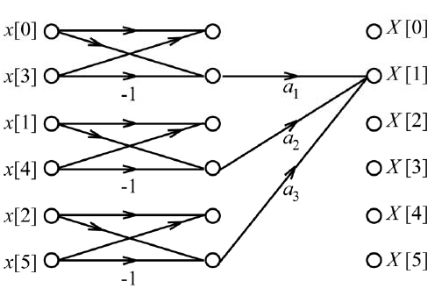
\includegraphics[width=0.5\columnwidth]{GATE/2019/EC/figs/q28.png}
        \caption{}
        \label{fig:q28}
    \end{figure}
    \begin{enumerate}
    \begin{multicols}{2}
        \item $a_{1}=-1$, $a_{2}=W_{6}$, $a_{3}=W_{6}^{2}$
        \item $a_{1}=1$, $a_{2}=W_{6}^{2}$, $a_{3}=W_{6}$
        \item $a_{1}=1$, $a_{2}=W_{6}$, $a_{3}=W_{6}^{2}$
        \item $a_{1}=-1$, $a_{2}=W_{6}^{2}$, $a_{3}=W_{6}$
    \end{multicols}
    \end{enumerate}

